% vim: set tw=0 linebreak:
\documentclass{beamer}
\usepackage{graphicx}
\usepackage{booktabs}
\usepackage{hyperref}
\hypersetup{pdfborder={0 0 0 0}}

% Reasonable themes:
% Antibes Bergen Berkeley Berlin Frankfurt Goettingen Ilmenau Luebeck Malmoe
% Montpellier PaloAlto Rochester Singapore Szeged Warsaw bars boxes
% compatibility default lined plain shadow sidebar split tree
% And these ones include the author's name on every slide:
% Berkeley

% Declare themes.
\mode<presentation>
\usetheme{UWHEP}

% Personal macros.
\newcommand{\email}[1]{{\texttt #1}}
\newcommand{\newframe}[1]{\section{#1}
    \frametitle{\sc{#1}}}
\newcommand{\subframe}[1]{\subsection{#1}
    \frametitle{\sc{#1}}}
\newcommand{\supers}[1]{\ensuremath{^\textrm{#1}}}
\newcommand{\subs}[1]{\ensuremath{_\textrm{#1}}}
\newcommand{\ca}{\ensuremath{\sim}}

% Author information.
\title{Site report: Wisconsin}
\author[Maier]{
    Sridhara Dasu \\
    Dan Bradley, Ajit Mohapatra, Will Maier
    {\tt \{dasu,dan,ajit,wcmaier\}@hep.wisc.edu}}
\institute[Wisconsin]{University of Wisconsin - High Energy Physics}
\date[2009.03.03]{USCMS T2 Workshop - LIGO Livingston, 2009.03.03}
\logo{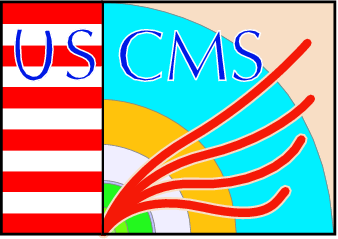
\includegraphics[height=0.6cm]{../../../Graphics/USCMS_logo.png}\hspace{.1cm}
\includegraphics[height=0.75cm]{../../../Graphics/UW_logo.png}}

\begin{document}

% - Hardware deployments for FY09: what is the plan for meeting this year's
% targets, and what are the estimated costs, including costs for doing
% necessary replacements of older hardware?
% -- Are there facility issues at the site that we need to be aware of for
% longer-term planning of T2 capabilities?
% -- Some sites do better than others on the various metrics (RSV, SAM, job
% robot, etc.), but why?  What does your site do that helps you meet targets
% on metrics, and for targets you don't meet, why not?  Would more operations
% support help you?

\begin{frame}
    \titlepage
\end{frame}

\section{Overview}
\begin{frame}
    \tableofcontents
\end{frame}

\section{2008-2009 Facilities Status}
\subsection{Batch}
\begin{frame}
% XXX: Use the following to generate N slots:
% condor_status -pool glow.cs.wisc.edu \
%   -constraint 'regexp("g[4-7]n\d+\.hep\.wisc\.edu", Machine)' \
%   -format '%s\n' Machine | wc -l
\begin{table}
\begin{tabular}{lrr}
    \toprule
    CPU Class               &   KSI2K   &   Slots \\
    \midrule
    2 x 2.80 GHz Xeon       &   210     &   110 \\  % g4-g7
    2 x 3.00 GHz Xeon       &   10      &   10 \\   % g8
    4 x 1.80 GHz Opteron    &   170     &   240 \\  % g9-g10
    8 x 2.66 GHz Xeon       &   180     &   120 \\  % g12
    8 x 3.00 GHz Xeon       &   250     &   260 \\  % g14
    \midrule
    Dedicated               &   820     &   740 \\
    Opportunistic           &   -       &   2460 \\
    \bottomrule
\end{tabular}
\caption{2008 Batch Status}
\label{2008_batch_status}
\end{table}

Since last workshop:
\begin{itemize}
    \item Added 32 8 x 3.00 GHz Xeon nodes
    \item Decommissioned 32 2 x 2.4 GHz Xeon
\end{itemize}
\end{frame}

\begin{frame}
\begin{figure}
    % http://noc.hep.wisc.edu/nrg/condor/pools/GLOW-condor-claimed.1yr.gif
    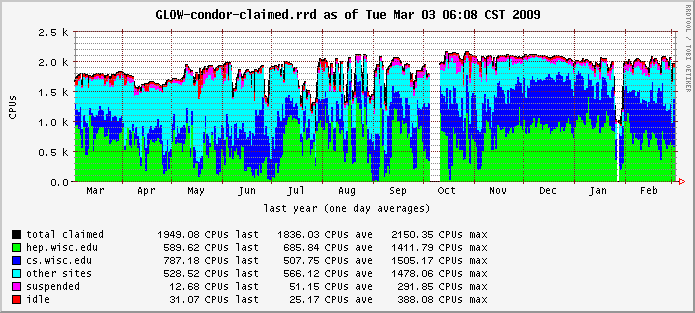
\includegraphics[width=\textwidth]{Graphics/GLOW-condor-claimed-1yr.png}
    \caption{Dedicated and opportunistic slots, 2008-2009}
\end{figure}
\end{frame}

\subsection{Storage}
\begin{frame}
\begin{table}
\begin{tabular}{lr}
    \toprule
    Dedicated       &   280 TB \\   % s5, s15 (10 * 24 TB)
    Dual-purpose    &   200 TB \\   % rest
    \midrule
    Raw             &   480 TB \\
    Replicated      &   240 TB \\
    \bottomrule
\end{tabular}
\caption{2008 Storage Status}
\label{2008_storage_status}
\end{table}

\begin{itemize}
    \item Added \ca{}300 TB since last workshop
    \item Both large, dedicated storage and dual-purpose machines
\end{itemize}
\end{frame}

\begin{frame}
\begin{figure}
    % XXX: hacked from makeplot.py in nod's (broken) ganglia webui stuff
    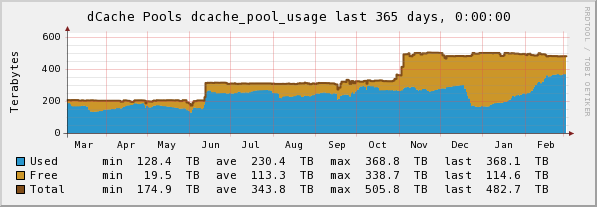
\includegraphics[width=\textwidth]{Graphics/dcache-usage-1yr.png}
    \caption{dCache usage, 2008-2009}
\end{figure}
\end{frame}

\subsection{Network}
\begin{frame}
\begin{figure}
    % XXX: http://stats.net.wisc.edu/cgi-bin/genstatspage.pl?db=r-csscplat-b380-3-core_vl369_bytes&time=1y
    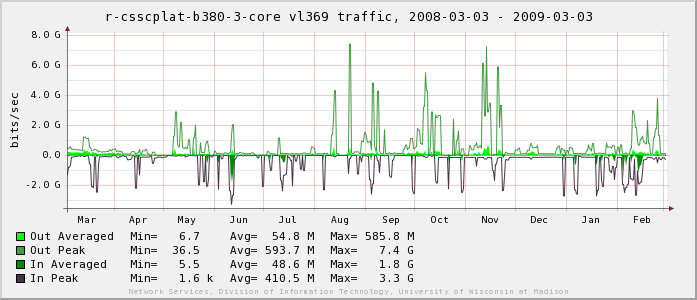
\includegraphics[width=\textwidth]{Graphics/network-1yr.png}
    \caption{WAN usage, 2008-2009}

\end{figure}
\begin{itemize}
    \item Tier2 traffic accounts for the majority of egress traffic from Wisconsin
    \item Ingress peaks due to PhEDEx transfers
\end{itemize}
\end{frame}

\section{2009 Deployment Plans}
\subsection{Batch and storage systems}
\begin{frame}
\begin{itemize}
    \item Target: NNN TB, NNN slots before 2010
    \item Deployment plan:
    \begin{itemize}
        \item March: 200 slots, 100TB
        \item June: \ca{}300TB
        \item September: 200 slots, 100TB
        \item December: \ca{}300TB
    \end{itemize}
\end{itemize}
\end{frame}

\subsection{Network}
\begin{frame}
\begin{figure}
    % XXX: hacked from makeplot.py in nod's (broken) ganglia webui stuff
    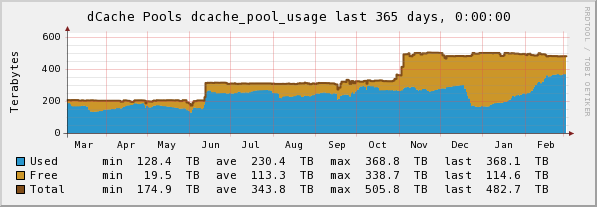
\includegraphics[width=\textwidth]{Graphics/dcache-usage-1yr.png}
    \caption{dCache usage, 2008-2009}
\end{figure}

\begin{itemize}
    \item \ldots{}
\end{itemize}
\end{frame}

\section{Facilities Planning}
\subsection{Cooling and Power}
\begin{frame}
\begin{itemize}
    \item At current capacity in new room
    \item Department building new room, will have access
    \item Can have space in the new room; sideeffect cooling
    % XXX: Plot
    \item Original room out of three-phase power
    \item Upgrade in progress, outlets available soon
\end{itemize}
\end{frame}

\subsection{Network}
\begin{frame}
\begin{itemize}
    \item Not at capacity, but typical egress flows much higher
    \item Largest consumer of campus bandwith
    \item Campus networking is interested in our case, offered to dynamically provision extra fiber as needed
    % XXX: Plot/doit plot
\end{itemize}
\end{frame}

\section{Metric Performance}
\subsection{SAM}
\begin{frame}
\begin{itemize}
    % XXX: plots
    \item \ldots{}
\end{itemize}
\end{frame}

\subsection{JobRobot}
\begin{frame}
\begin{itemize}
    % XXX: plots
    \item \ldots{}
\end{itemize}
\end{frame}

\subsection{RSV}
\begin{frame}
\begin{itemize}
    % XXX: plots
    \item \ldots{}
\end{itemize}
\end{frame}

\end{document}
